
Depuis la démocratisation de l'informatique et plus particulièrement
de la cartographie sur le web, il n'a jamais été aussi facile de
trouver ou de partager une position géographique. On peut désormais
facilement connaitre les coordonnées, dans un système de référence
donné, d'un bâtiment situé à l'autre bout de la terre ou de la rue, ce
qu'aucune personne ne pourrait faire. Mais ces systèmes seraient bien
incapables de comprendre une position telle que nous la décrivons a
quelqu’un demandant son chemin (\eg \enquote{Prenez la première à
  droite après la boulangerie}). Pourtant les coordonnées, comme une
description orale d'un itinéraire ou d'un endroit décrivent tout deux
la même chose : une position dans l'espace. La différence entre ces
deux approches tient dans la manière dont elles décrivent une
position. Les coordonnées définissent un référentiel dit
\enquote{direct} alors qu'une description orale de position correspond
a un référentiel indirect, où la position des objets est exprimée à
travers des relations avec d'autres objets. Si l’interprétation d'une
position exprimée dans un référentiel direct ne pose que peu de
problèmes, une fois le référentiel connu, il n'en va pas de même pour
les positions exprimées dans un référentiel indirect.

L'interprétation automatisée de telles descriptions est un sujet de
recherche dynamique, puisque c'est la principale manière qu'utilisent
les êtres humains pour décrire une position. De nombreux domaines
peuvent bénéficier d'une interprétation automatisée de descriptions de
positions, par exemple les humanités numériques, qui peuvent exploiter
ces techniques pour localiser des événements ou des lieux mentionnés
dans des corpus d'archives historiques. Mais de telles possibilités
présentent également des intérêts hors du domaine de la recherche. Un
des domaines d’application étudié est l'assistance aux secours; le
domaine d’application de cette thèse. Les secours à la personne sont
régulièrement amenés à intervenir dans des zones imparfaitement
définies, notamment lorsque aucun témoin n'est capable de donner une
description satisfaisante de sa position.




% La transformation d'une description de position en une zone définie
% par des coordonéess



% %-> transition secours en montagne "le problème devient grave"

% La difficulté de cette opération peut devenir contraignante lorsque la
% rapidité de la localisation est indispensable, notamment dans les
% secours a la personne. Plusieurs travaux ont donc cherché a améliorer
% le processus de

% \autocite{DosSantosFerreria2019} 

% -> transition choucas
Cette difficulté de localisation des victimes est d'autant plus
important lorsqu'il est nécessaire de localiser des personnes perdues
dans des espaces offrant peu de points de repères identifiables sans
ambiguïté. C'est, par exemple, le cas pour les unités de secours en
montagne \acp{usem}, qui sont régulièrement amenés à secourir des
personnes perdues ou blessées en montagne. Pour ces unités le problème
de la difficulté de localisation est accentué par ces
implications. Les \ac{usem} disposant de moyens humains et matériels
limités, la focalisation sur une alerte peut impacter aussi bien
l'opération de secours en cours, que les potentielles opérations à
venir, qui pourraient être retardées.

Pour faciliter la localisation des victimes en montagne les
secouristes du \ac{pghm} de Grenoble ont développé une solution,
Gend'Loc, permettant de localiser le requérant (\ie la personne
appelant les secours) à l'aide du GPS intégré a son téléphone
portable. Cette solution à l'avantage de permettre une localisation
rapide et assez facile à utiliser pour le requérant, mais elle a
l'inconvénient majeur d'être dépendante du téléphone du requérant et
de son bon fonctionnement. De nombreux facteurs peuvent rendre cette
solution inopérante, notamment lorsque le requérant ne dispose pas
d'un téléphone avec GPS, lorsque les secours sont contactés par un
tiers ou lorsque la victime n'arrive pas à effectuer la manipulation
nécessaire. Dans ces situations les secouristes n'ont d'autres choix
que d'identifier la position du requérant manuellement, en recoupant
les informations qui leur sont données avec leurs connaissances
personnelles et les données géographiques qu'ils ont à leur
disposition. Le résultat de ce processus est assez variable: si les
secouristes peuvent parvenir à identifier très rapidement la position
de la victime a l'aide de quelques éléments très discriminants, il est
parfois difficile pour la victime de donner des informations qui
soient suffisamment claires ou discriminantes pour que les secouristes
puissent les interpréter. Dans ces conditions, la phase de
localisation peut devenir extrêmement longue et critique.

Le projet de recherche Choucas \footnote{Projet ANR-16-CE23-0018.} a
été initié dans le but de développer des solutions permettant de
faciliter le traitement de ces alertes spécifiques. L'hypothèse
première de ce projet est que la géomatique et ses méthodes peuvent
aider à identifier les zones correspondant aux informations données
par les victimes. En effet, de nombreuses méthodes qui ont été
proposées dans le domaine de la géomatique pourraient être employés a
cet effet. Par exemple les travaux autour des questions de visibilité
pourraient être exploités pour identifier la position d'un requérant
décrivant son champ de vision, les travaux sur la modélisation de
trajectoire pourraient être utilisés pour localiser une personne
indiquant qu'elle a suivi un itinéraire donné, \emph{etc.} Un tel
objectif n'est cependant pas réalisable par la \enquote{simple}
concaténation de méthodes préexistantes et impose de travailler à
l'étude et a l’enrichissement des données utilisables par les
secouristes, de définir des solutions leur permettant d’interagir avec
les solutions développées au sein du projet, d'étudier les subtilités
et les spécificités des descriptions de localisation en milieux
montagneux, \emph{etc.}

% Présentaiont thèse
Notre thèse se rattache spécifiquement à ce dernier point. Plus
précisément, notre objectif est de proposer une méthode permettant de
construire les zones correspondant aux descriptions de positions
données par les requérants. Notre but n'est cependant pas de créer un
\enquote{secouriste virtuel}, réalisant l'ensemble des tâches
effectuées manuellement par ces derniers et interprétant
automatiquement le discours du requérant, mais de proposer une méthode
d'assistance, facilitant l'identification des zones correspondant à
une description de position.

Cet objectif induit de nombreuses difficultés, la première d'entre
elles étant la taille de l'espace des possibles. Une personne
décrivant sa position peut être amenée à utiliser de nombreux
éléments, parfois très différents, comme son itinéraire, sa position
de départ, son objectif visé, décrire son champ de vision, \emph{etc.}
L'identification de la position du requérant impose donc d'être en
capacité de pouvoir interpréter une majorité, sinon toutes les
informations qu'elle donne. De plus nous devons être en mesure de
combiner ces différentes informations de manière identifier la
position qu'elles décrivent conjointement.

% inteprétation sémantique
La seconde difficulté est d'être en capacité d'interpréter les
concepts utilisés dans leur discours par les requérants. Si nous ne
cherchons pas à interpréter directement le discours du secouriste
celui-ci décrit sa position en employant des concepts issus du langage
naturel (\eg \enquote{à côté de}, \enquote{en face de},
\emph{etc.}). Or ces derniers peuvent voir leur signification varier
en fonction du contexte, de l'objet auquel ils se réfèrent,
\emph{etc.}  Nous devons donc être en capacité d'identifier les
différents sens que peuvent avoir ces concepts et identifier les
situations dans lesquelles ils sont utilisés. Par ailleurs ces
concepts peuvent voir leur signification impactée par le fait que
notre cas d’application soit spécifique au milieu montagneux.

% prise en compte imprécision
Un autre problème lié à l'interprétation de ces concepts est qu'ils
peuvent être vagues.  Il est, par exemple, difficile de fixer la
limite entre ce qui est proche et ce qui est éloigné, et l'on peut
s'attendre a ce que deux personnes n'aient pas exactement la même
utilisation de ces concepts. L’identification de la zone correspondant
à une description de position ne nécessite donc pas que d'interpréter
correctement les concepts utilisés, mais également de prendre en
compte leur imprécision.

% incertitude
Indépendamment de leur imprécision, les informations données par les
victimes peuvent également êtres faussées. Il est par exemple possible
qu'elles se trompent dans le nom d'un point leur servant de reprère ou
qu'elles fassent des confusions. Lorsque ces erreurs sont manifestes
le secouriste peut les identifier et les corriger, mais ce n'est pas
toujours possible. Il est donc nécessaire de proposer une méthode qui
puisse tenir compte de la fiabilité variable des informations données.

%\begin{figure}
%   \centering
%   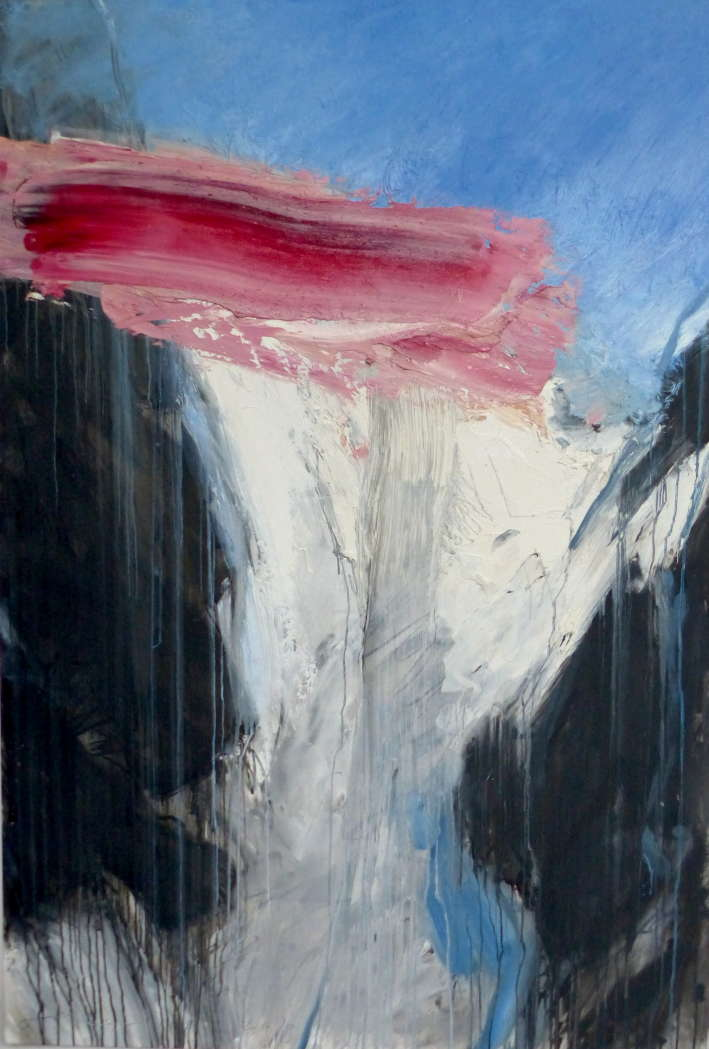
\includegraphics{./figures/Le_couloir_Rochette.jpg}
%   \caption{\emph{Le couloir,} Jean-Marc \bsc{Rochette,} 2010.}
%   \label{fig:couloir_rochette}
% \end{figure}

\addsec{Organisation du manuscrit}

Notre mémoire de thèse est organisé en trois parties, totalisant neufs
chapitres. Dans la \autoref{part:01} nous présenterons le cadre
général dans lequel notre travail s'inscrit. Le premier chapitre sera
dédié a la présentation du contexte applicatif et organisationnel de
cette thèse. Nous détaillerons le rôle et le fonctionnement des
secours en montagne, les problèmes soulevés par la localisation des
victimes et la manière dont le projet CHOUCAS souhaite y répondre. Le
second chapitre est destiné à présenter le contexte de scientifique et
la problématisation de notre thèse. Enfin, dans le troisième chapitre
nous dresserons un état de l'art sur les questions principales de ce
travail.

La \autoref{part:02} est destinée à présenter notre méthode de
transformation des positions exprimées dans un référentiel indirect en
des zones de localisation. Elle est constituée de cinq chapitres. Le
premier chapitre de cette partie présente l’organisation générale de
notre méthode (\autoref{chap:04}). Les chapitres suivants
approfondissent des points spécifiques de cette méthode. Dans le
\autoref{chap:05} nous détaillerons le fonctionnement de la première
phase de la méthode, \emph{la décomposition.} Le \autoref{chap:06}
sera quant à lui consacré a la définition d'un modèle permettant la
représentation d'objets géographiques imprécis, tels que ceux produits
par notre méthode. Dans le \autoref{chap:07} nous présenterons la
seconde phase de notre méthode, \emph{la spatialisation.} Le dernier
chapitre de cette seconde partie sera consacré à la présentation de la
dernière phase de notre méthode, la \emph{fusion.}

Enfin, la \autoref{part:03} de ce manuscrit présente l’application de
la méthode définie a plusieurs alertes réelles. Cette partie ne
contient qu'un seul chapitre, le neuvième, où notre méthode est
appliquée à la modélisation de deux alertes réelles. Nous y
détaillerons la mise en œuvre de notre méthode sur ces alertes et
analyserons les résultats obtenus.

Pour finir, nous conclurons classiquement ce manuscrit par un bilan
des contributions et des perspectives.


%%% Local Variables:
%%% mode: latex
%%% TeX-master: "../../main"
%%% End:
